%% LyX 2.0.2 created this file.  For more info, see http://www.lyx.org/.
%% Do not edit unless you really know what you are doing.
\documentclass[english]{article}
\usepackage[T1]{fontenc}
\usepackage[latin9]{inputenc}
\usepackage{float}
\usepackage{graphicx}
\usepackage{babel}
\begin{document}

\title{Test of error calculations for Ising model in 1D and 2D}

\maketitle
This is short theoretical explanation of the test: \textbf{IsingTestError1D.h}
and \textbf{IsingTestError2D.h}.


\section{Standard deviation}

\medskip{}


In files IsingTestError1D.h and IsingTestError2D.h we test function\linebreak{}
\textit{Ising::ERROR(string totalFname, ISING\_ERROR\_TYPE error\_type)
}which calculates standard daviation of choosen variable $X$ using
bootstrap algorithm. 

\medskip{}


Standard deviation of variable $X$ can be expressed by:

\[
\sigma(X)=\sqrt{\langle(X-\langle X\rangle)^{2}\rangle}=\sqrt{\langle X^{2}\rangle-\langle X\rangle^{2}}
\]


and it tells as how far a set of numbers is spread out. Low standard
deviation indicates that the data points tend to be near the mean
value of the set, high - the opposite. Apart fom showing dispersion
of a data set, standard deviation is usually used as a measure of
confidence in statistical conclusions. 

The standard deviation of some data set is a square root of its variance
$V(X)=\langle X^{2}\rangle-\langle X\rangle^{2}$ . A useful property
of the standard deviation is that, unlike the variance, it is expressed
in the same units as the data.


\section{Bootstrap method}

\medskip{}


If the sample size is insufficient to calculate the standard deviation
from definition, we can use for this purpose bootstrap method. Bootstraping
uses approximate distribution to estimate properties of an estimator
(like standard deviation). To achieve it we can take set of observed
data and (assuming independence of observation) construct a number
of resamples. Such resamples have to be of equal size to the observed
dataset and be obtained by random sampling with replacement from the
original dataset. From a number of resamples we can create approximate
distribution of variable and obtain estimator - in our case standard
deviation.

\medskip{}


The general bootstrap algorithm is as follows:
\begin{enumerate}
\item Let $n$ be a number of elements in dataset. Pick at random $n$ elements
(with returns). 
\item Calculate an observable $X$ using $n$ elements created in 1. 
\item Repeat 1. and 2. $m$ times. This gives a series $X_{1}$, $X_{2}$,
..., $X_{m}$ of estimations of $X$. 
\item Use this series to calculate the standard deviation $\sigma=\sqrt{\langle X^{2}\rangle-\langle X\rangle^{2}}$
.
\end{enumerate}
\medskip{}


We specifically want to use this algorithm for calculation of standard
deviation of such physical quantities as specific heat $C$, magnetic
susceptibility $\chi$ etc. However, as our Monte Carlo simulations
are time- and memory-consuming, it's difficult to obtain suffiecient
set of such quantities for calculating standard deviation. Instead
we use data from one Monte Carlo simulation to construct set of resamples,
from each we calculate the necessary quantity and find standard deviation
of obtained distribution. 

\medskip{}


At this stage of project calculation of standard deviation of 3 quantities
are implemented: 
\begin{itemize}
\item specific heat $C$,
\item magnetic susceptibility $\chi$,
\item magnetisation $M$.
\end{itemize}
You can choose proper quantity by choosing argument\textit{ error\_type
}in function \textit{Ising::ERROR} as ERROR\_CHI, ERROR\_CC or ERROR\_OP.


\section{Tests}

\medskip{}


In the tests IsingTestError1D.h and IsingTestError2D.h we calculate
error (standard deviation) of magnetic susceptibility in function
of production time. We use bootstrap method implemented in function
\textit{Ising::ERROR}. 

General result for error known in MC integration methods is inversely
proportionate to square root of number of samples $n$:

\[
error\propto1/\sqrt{n}
\]


Therefore, we expect our error would diminish with increase of production
time like $1/\sqrt{prod\_t}$. Results agree with our predictions.
On figures below you can see calculated error in function of production
time as well as fits proportionate to $1/\sqrt{prod\_t}$.

\medskip{}


\begin{figure}[H]
\begin{centering}
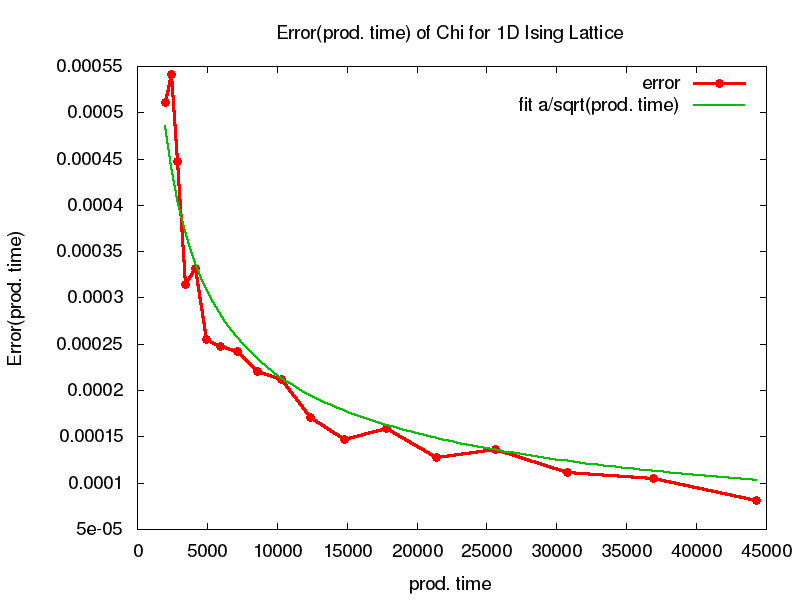
\includegraphics[scale=0.2]{IsingTestError1D}
\par\end{centering}

\caption{Error (standard deviation) of magnetic susceptibility in function
of production time for 1D Ising lattice.}
\end{figure}


\begin{figure}[H]
\begin{centering}
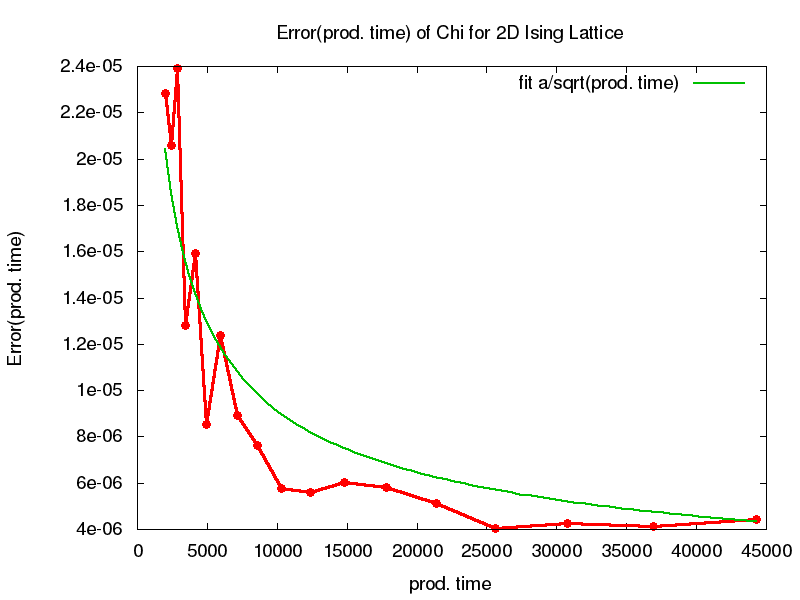
\includegraphics[scale=0.2]{IsingTestError2D}
\par\end{centering}

\caption{Error (standard deviation) of magnetic susceptibility in function
of production time for 2D Ising lattice.}
\end{figure}


\medskip{}


\medskip{}


Additionally we calculate error of magnetic susceptibility in function
of temperature and compare it with difference between analytical and
numerical solution for $\chi$. We do it only for 1D case because
we do not now exact formula for $\chi$ in 2D. We can see both error
and shown difference decrease with temperature and are of the same
order of magnitude.

\medskip{}


\begin{center}
\begin{figure}[H]
\begin{centering}
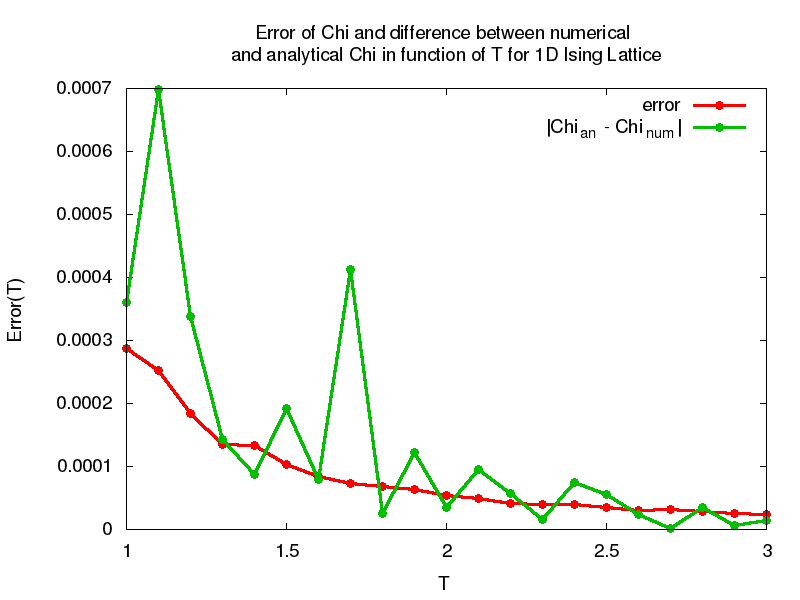
\includegraphics[scale=0.2]{IsingTestError1D_T}
\par\end{centering}

\caption{Comparison of error (standard deviation) and difference of analytical
and numerical magnetic susceptibility in function of temperature.}
\end{figure}

\par\end{center}
\end{document}
